\begin{pastexam}[label={px:ncku-112-prog-13}]{成大資訊聯招 112 學年度 第 13 題}
（追蹤）

(10\%) Illustrate the operation of HEAPSORT on the array $S$=[5, 13, 2, 25, 7, 17, 20, 8, 4]
\end{pastexam}

\begin{pastsoln}
約定：照資結書第~14.6~節的 \proc{Heapsort}（資結書虛擬碼~14.13）：先用
\proc{Build-Max-Heap} 由下而上建最大堆積，再反覆把根換到尾端、堆積大小減一、對根做
\proc{Sift-Down}。 下沉時兩個子節點相等就換左邊（本題沒有相等的數）。 $n = 9$，陣列從 $1$
開始。

\textbf{建堆積}：$i$ 從 $\lfloor 9/2 \rfloor = 4$ 做到 $1$，每一列是那一次下沉之後的陣列。
\begin{center}
\small
\begin{tabular}{lc*{9}{c}}
\toprule
& 交換 & 1 & 2 & 3 & 4 & 5 & 6 & 7 & 8 & 9 \\
\midrule
開始 & & 5 & 13 & 2 & 25 & 7 & 17 & 20 & 8 & 4 \\
$i = 4$ & 0 & 5 & 13 & 2 & 25 & 7 & 17 & 20 & 8 & 4 \\
$i = 3$ & 1 & 5 & 13 & 20 & 25 & 7 & 17 & 2 & 8 & 4 \\
$i = 2$ & 1 & 5 & 25 & 20 & 13 & 7 & 17 & 2 & 8 & 4 \\
$i = 1$ & 3 & 25 & 13 & 20 & 8 & 7 & 17 & 2 & 5 & 4 \\
\bottomrule
\end{tabular}
\end{center}
$i = 4$：$25$ 比子節點 $8$、$4$ 大，不動。 $i = 3$：$2$ 和較大的子節點 $20$ 交換。 $i = 2$：
$13$ 和 $25$ 交換，到位置 4 後比 $8$、$4$ 大，停。 $i = 1$：$5$ 依序和 $25$、$13$、$8$ 交換，
停在位置 8。 建好的堆積：

\begin{center}
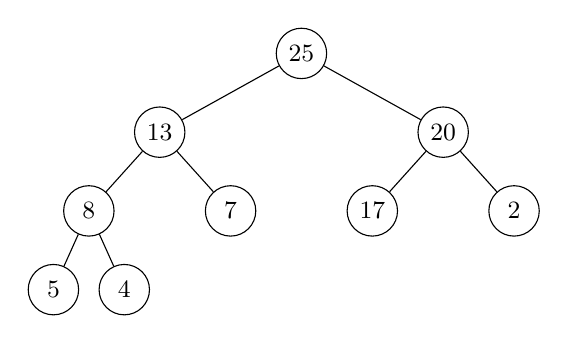
\begin{tikzpicture}[level distance=10mm,
  every node/.style={circle,draw,inner sep=0pt,minimum size=6.4mm,font=\small},
  level 1/.style={sibling distance=36mm}, level 2/.style={sibling distance=18mm},
  level 3/.style={sibling distance=9mm}]
\node {25}
  child {node {13} child {node {8} child {node {5}} child {node {4}}} child {node {7}}}
  child {node {20} child {node {17}} child {node {2}}};
\end{tikzpicture}
\end{center}

\textbf{排序}：每一列是排序迴圈（取出根、下沉）做完一輪之後的陣列，「交換」是那一次下沉交換了幾次，灰
色是已經排好、不在堆積裡的格子。
\begin{center}
\small
\begin{tabular}{lc*{9}{c}}
\toprule
& 交換 & 1 & 2 & 3 & 4 & 5 & 6 & 7 & 8 & 9 \\
\midrule
建好堆積 & & 25 & 13 & 20 & 8 & 7 & 17 & 2 & 5 & 4 \\
取出 25 & 2 & 20 & 13 & 17 & 8 & 7 & 4 & 2 & 5 & {\color{black!40}25} \\
取出 20 & 1 & 17 & 13 & 5 & 8 & 7 & 4 & 2 & {\color{black!40}20} & {\color{black!40}25} \\
取出 17 & 2 & 13 & 8 & 5 & 2 & 7 & 4 & {\color{black!40}17} & {\color{black!40}20} & {\color{black!40}25} \\
取出 13 & 2 & 8 & 7 & 5 & 2 & 4 & {\color{black!40}13} & {\color{black!40}17} & {\color{black!40}20} & {\color{black!40}25} \\
取出 8 & 1 & 7 & 4 & 5 & 2 & {\color{black!40}8} & {\color{black!40}13} & {\color{black!40}17} & {\color{black!40}20} & {\color{black!40}25} \\
取出 7 & 1 & 5 & 4 & 2 & {\color{black!40}7} & {\color{black!40}8} & {\color{black!40}13} & {\color{black!40}17} & {\color{black!40}20} & {\color{black!40}25} \\
取出 5 & 1 & 4 & 2 & {\color{black!40}5} & {\color{black!40}7} & {\color{black!40}8} & {\color{black!40}13} & {\color{black!40}17} & {\color{black!40}20} & {\color{black!40}25} \\
取出 4 & 0 & 2 & {\color{black!40}4} & {\color{black!40}5} & {\color{black!40}7} & {\color{black!40}8} & {\color{black!40}13} & {\color{black!40}17} & {\color{black!40}20} & {\color{black!40}25} \\
\bottomrule
\end{tabular}
\end{center}
以第一輪為例：$25$ 和 $A[9] = 4$ 交換，堆積大小變成 $8$；$4$ 在根，子節點 $13$、$20$，和
$20$ 交換；到位置 3，子節點 $17$、$2$，和 $17$ 交換；到位置 6，子節點的位置 $12$ 超過堆積
大小，停。 共交換 $2$ 次。 第二輪 $20$ 和 $A[8] = 5$ 交換，$5$ 下沉時子節點是 $13$、$17$，換
$17$；到位置 3，子節點 $4$、$2$ 都比 $5$ 小，停，只交換 $1$ 次。

結果：$S = [2, 4, 5, 7, 8, 13, 17, 20, 25]$。 檢查：每一列前面那段都滿足
$A[i] \ge A[2i]$、$A[2i + 1]$，後面灰色的那段由小到大，而且都不小於前面那段的任何數。
\end{pastsoln}
